\documentclass[11pt,border=2mm]{standalone}
\usepackage{csquotes}
\usepackage[backend=biber,style=numeric,sorting=none]{biblatex}

\providecommand{\FigScale}{1}
 
\usepackage{siunitx}
\usepackage{tikz}
\usetikzlibrary{decorations.pathmorphing,patterns}
\usetikzlibrary{shapes.geometric, arrows}
\usetikzlibrary{positioning}
 
\usepackage{amsmath}
 
\usepackage{tikz-3dplot}
\usetikzlibrary{3d}
 
\usepackage[siunitx,american]{circuitikz}
 
\usepackage{pgfplots}
\usepgfplotslibrary{units}
\usepgfplotslibrary{groupplots}
\pgfplotsset{compat=1.14}
 
\ctikzset{tripoles/mos style/arrows}
 


\begin{document}

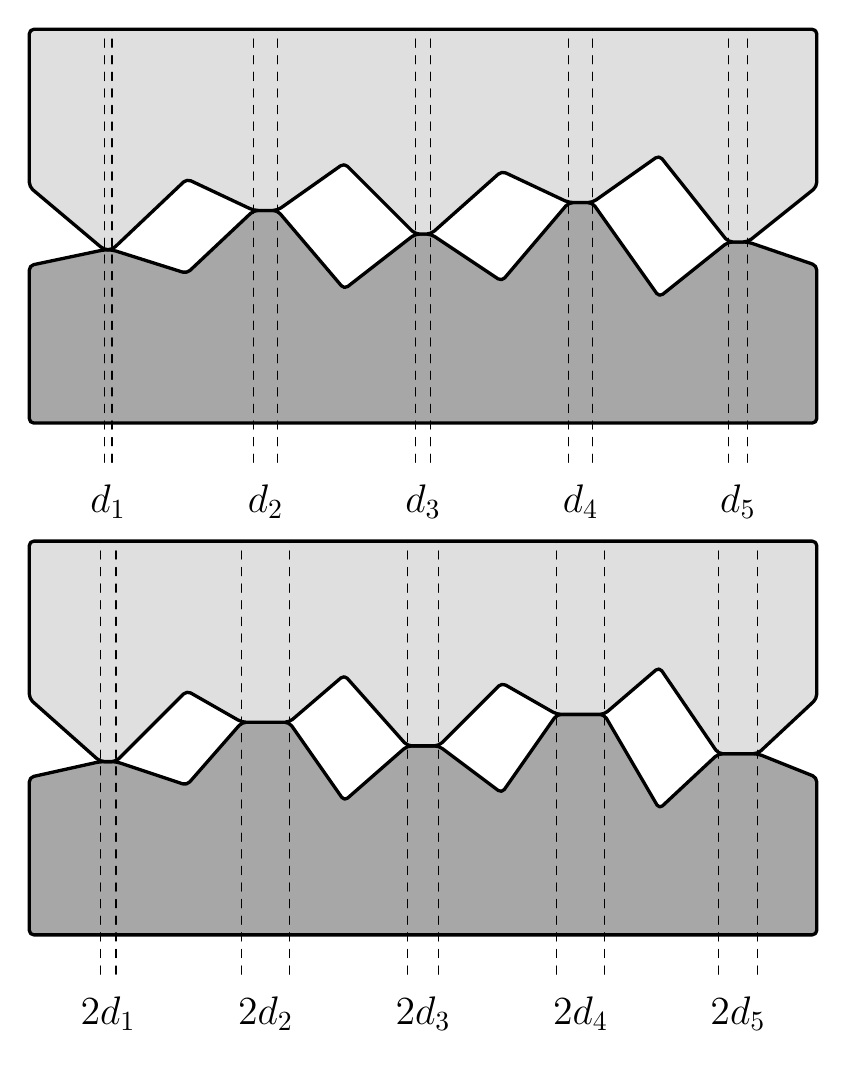
\begin{tikzpicture}[scale=\FigScale, line join=round, line cap=round]

\definecolor{IBM1}{HTML}{648fff}
\definecolor{IBM2}{HTML}{785ef0}
\definecolor{IBM3}{HTML}{dc267f}
\definecolor{IBM4}{HTML}{fe6100}
\definecolor{IBM5}{HTML}{ffb000}
\definecolor{IBM6}{HTML}{d55e00}
\definecolor{IBM7}{HTML}{cc79a7}
\definecolor{IBM8}{HTML}{0072b2}
\definecolor{IBM9}{HTML}{f0e442}
\definecolor{IBM10}{HTML}{009e73}

\draw[very thick, fill=gray!69, rounded corners=1.6pt]
(0,0)--(10,0)--(10,2)--(9.125,2.3)--(8.875,2.3)--(8,1.6)--(7.15,2.8)--(6.85,2.8)--(6,1.8)--(5.1,2.4)--(4.9,2.4)--(4,1.7)--(3.15,2.7)--(2.85,2.7)--(2,1.9)--(1.05,2.2)--(0.95,2.2)--(0,2)--cycle;

\draw[very thick, fill=gray!25, rounded corners=1.6pt]
(0,5)--(10,5)--(10,3)--(9.125,2.3)--(8.875,2.3)--(8,3.4)--(7.15,2.8)--(6.85,2.8)--(6,3.2)--(5.1,2.4)--(4.9,2.4)--(4,3.3)--(3.15,2.7)--(2.85,2.7)--(2,3.1)--(1.05,2.2)--(0.95,2.2)--(0,3)--cycle;

\draw[dashed](9.125,-0.5)--(9.125,5);
\draw[dashed](8.875,-0.5)--(8.875,5);
\node[] at (9,-1) {\Large{$d_5$}};
\draw[dashed](7.15,-0.5)--(7.15,5);
\draw[dashed](6.85,-0.5)--(6.85,5);
\node[] at (7,-1) {\Large{$d_4$}};
\draw[dashed](5.1,-0.5)--(5.1,5);
\draw[dashed](4.9,-0.5)--(4.9,5);
\node[] at (5,-1) {\Large{$d_3$}};
\draw[dashed](3.15,-0.5)--(3.15,5);
\draw[dashed](2.85,-0.5)--(2.85,5);
\node[] at (3,-1) {\Large{$d_2$}};
\draw[dashed](1.05,-0.5)--(1.05,5);
\draw[dashed](0.95,-0.5)--(0.95,5);
\node[] at (1,-1) {\Large{$d_1$}};

\begin{scope}[yshift=-6.5cm]
\draw[very thick, fill=gray!69, rounded corners=1.6pt]
(0,0)--(10,0)--(10,2)--(9.25,2.3)--(8.75,2.3)--(8,1.6)--(7.3,2.8)--(6.7,2.8)--(6,1.8)--(5.2,2.4)--(4.8,2.4)--(4,1.7)--(3.3,2.7)--(2.7,2.7)--(2,1.9)--(1.1,2.2)--(0.9,2.2)--(0,2)--cycle;

\draw[very thick, fill=gray!25, rounded corners=1.6pt]
(0,5)--(10,5)--(10,3)--(9.25,2.3)--(8.75,2.3)--(8,3.4)--(7.3,2.8)--(6.7,2.8)--(6,3.2)--(5.2,2.4)--(4.8,2.4)--(4,3.3)--(3.3,2.7)--(2.7,2.7)--(2,3.1)--(1.1,2.2)--(0.9,2.2)--(0,3)--cycle;

\draw[dashed](9.25,-0.5)--(9.25,5);
\draw[dashed](8.75,-0.5)--(8.75,5);
\node[] at (9,-1) {\Large{$2d_5$}};
\draw[dashed](7.3,-0.5)--(7.3,5);
\draw[dashed](6.7,-0.5)--(6.7,5);
\node[] at (7,-1) {\Large{$2d_4$}};
\draw[dashed](5.2,-0.5)--(5.2,5);
\draw[dashed](4.8,-0.5)--(4.8,5);
\node[] at (5,-1) {\Large{$2d_3$}};
\draw[dashed](3.3,-0.5)--(3.3,5);
\draw[dashed](2.7,-0.5)--(2.7,5);
\node[] at (3,-1) {\Large{$2d_2$}};
\draw[dashed](1.1,-0.5)--(1.1,5);
\draw[dashed](0.9,-0.5)--(0.9,5);
\node[] at (1,-1) {\Large{$2d_1$}};

\end{scope}

\end{tikzpicture}

\end{document}